Gravitons could be produced in proton-proton collisions at the \gls{lhc}. The
interaction Lagrangian is given by~\cite{ADDPhenomenology}:
\begin{equation}
  \label{eq:114}
  \mathcal{L} = - \frac{1}{\overbar{M}_P} G^{(n)}_{\mu\nu} T^{\mu\nu}
\end{equation}
where $\overbar{M}_P = M_P/\sqrt{8 \pi}$ is the reduced Planck mass,
$G^{(n)}_{\mu\nu}$ is the graviton field in $n$ dimensions and $T^{\mu\nu}$ is
the stress-energy tensor, and thus the graviton production cross section is
suppressed by a factor $1/\overbar{M}^2_P$. Nevertheless the mass splitting of
the Kaluza-Klein modes is given by~\cite{ADDPhenomenology}:
\begin{equation}
  \label{eq:115}
  \Delta m \approx \frac{1}{R} = \md \left( \frac{\md}{\overbar{M}_P}
  \right)^{2/n} \approx \left( \frac{\md}{\mathrm{TeV}} \right)^{\frac{n +
  2}{2}} 10^{\frac{12 n - 31}{n}}~\mathrm{eV}
\end{equation}
where $n$ represents the extra dimensions which for $\md = 1$~TeV and $n =$ 4,
6, 8 gives $\Delta m = 20$~keV, 7~MeV and 0.1~GeV. For $n > 6$ only few \gls{kk}
modes can be produced and the total production cross section becomes
negligible~\cite{ADDPhenomenology} while only for a large number of extra
dimensions the mass splitting energy becomes comparable with the experimental
energy resolution and the number of \gls{kk} modes produced is capable of
compensating the $1/\overbar{M}^2_p$ suppression factor in the production cross
section. The graviton lifetime of
$\tau_G \approx \overbar{M}^2_P/m^3 \approx (\mathrm{TeV}/m)^3 \approx
10^3$~seconds~\cite{ADDPhenomenology} makes it stable over \gls{atlas} detection
time. The $1/\overbar{M}^2_p$ suppression factor can be interpreted as the low
probability that a graviton propagating in the extra dimensions crosses the
usual three spatial dimensions~\cite{ADDPhenomenology}. The Kaluza-Klein
graviton only interacts weakly through the gravitational interaction with the
Standard Model particles and thus behaves like a non interacting, massive and
stable particle which, escaping detection, leads to an energy imbalance in the
detector which can be investigated using the monojet
signature. \cref{fig:add_feynman} shows the three main graviton production modes
at \gls{lhc}. These production modes are implemented at \gls{lo} in the Monte
Carlo generator PYTHIA8~\cite{PYTHIA8}.

As mentioned earlier, collider searches do not have sensitivity to \gls{add}
scenarios with more than six extra dimensions, for this reason in this analysis
only models with six or less extra dimensions are considered. Moreover, since
from \cref{eq:69}, using n = 1 leads to $R \approx 10^{11}$~m which is
empirically excluded~\cite{ADDPhenomenology}, only models with two extra
dimensions or more are considered. Finally in the case with two and three extra
dimensions, values of $\md$ lower than 110~TeV and 5~TeV respectively are
excluded by cosmological arguments~\cite{ADDCosmology}.

The signal samples used to calculate the exclusion limits on $\md$ are generated
with PYTHIA8. The following relation between the production cross section and
$\md$~\cite{ADDPhenomenology} was verified with PYTHIA samples and is exploited
in order to generate only a single Monte Carlo sample per number of dimensions:
\begin{equation}
  \label{eq:116}
  \sigma_\mathrm{nom} = \frac{C_n}{{(\md^\mathrm{nom})}^{n + 2}}
\end{equation}
where $\sigma_\mathrm{nom}$ and $\md^\mathrm{nom}$ are the nominal values of the
cross section and the Planck scale used in PYTHIA8 to generate the \gls{mc}
signal sample while $C_n$ is a constant term for a given center of mass energy
and number of extra dimensions that is determined from \cref{eq:116} as:
\begin{equation}
  \label{eq:179}
  C_n = \sigma_\mathrm{nom} {(\md^\mathrm{nom})}^{n + 2}.
\end{equation}
Thus a single Monte Carlo sample is generated for each $n$ and the \gls{add}
graviton cross section can be deduced for any $\md$ from that relation. The
samples generated along with $\sigma_\mathrm{nom}$ and $\md_\mathrm{nom}$ used
in this analysis are reported in \cref{tab:sigma_md_ref}. Once the value of
$C_n$ is determined, \cref{eq:116} can be regarded as a function $\sigma(\md)$
and the cross section is set by the Planck scale. In particular, for some
excluded value of $\md^\mathrm{excl}$:
\begin{equation}
  \label{eq:180}
  \frac{\sigma_\mathrm{nom}}{\sigma_\mathrm{excl}} = \left(
    \frac{\md^\mathrm{excl}}{\md^\mathrm{nom}} \right)^{n + 2}.
\end{equation}
From the definition of excluded signal strength
$\mu_\mathrm{excl} = \sigma/\sigma_\mathrm{nom}$ where $\sigma$ is the
production cross section of some \gls{bsm} model, we have that:
\begin{equation}
  \label{eq:181}
  \sigma_\mathrm{excl} = \mu_\mathrm{excl} \sigma_\mathrm{nom}
\end{equation}
from which:
\begin{equation}
  \label{eq:182}
  \mu_\mathrm{excl} = \left( \frac{\md^\mathrm{nom}}{\md^\mathrm{excl}}
  \right)^{n + 2}
\end{equation}
and finaly:
\begin{equation}
  \label{eq:117}
  \md^\mathrm{excl} = \frac{\md^\mathrm{nom}}{\mu^{1/(n + 2)}_\mathrm{excl}}.
\end{equation}
With this prescription upper limits on the signal strength are translated into
upper limits on the fundamental Planck scale $\md$.
\begin{table}[!h]
  \centering
  \begin{tabular}{lcc}
    \toprule
    \multicolumn{3}{c}{Nominal Cross Section and Planck Scale Values} \\
    \midrule \midrule
    Model & $\md$~[GeV] & $\sigma$~[pb] \\
    \midrule
    ADD n = 2 & 5300 & 1.55 \\
    ADD n = 3 & 4100 & 1.82 \\
    ADD n = 4 & 3600 & 2.29 \\
    ADD n = 5 & 3200 & 4.18 \\
    ADD n = 6 & 3000 & 7.22 \\
    \bottomrule
  \end{tabular}
  \caption{Reference values for the cross section and the Planck scale used to
    generate the \gls{add} signal samples at 13~TeV.}
  \label{tab:sigma_md_ref}
\end{table}
\begin{figure}[!h]
  \centering
  \begin{subfigure}{.48\linewidth}
    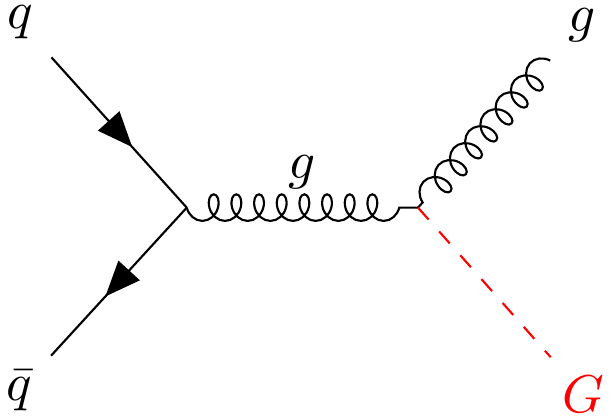
\includegraphics[width=\linewidth]{qq_to_gG}
    \caption{$q \bar{q} \rightarrow g G$.}
  \end{subfigure}
  \begin{subfigure}{.48\linewidth}
    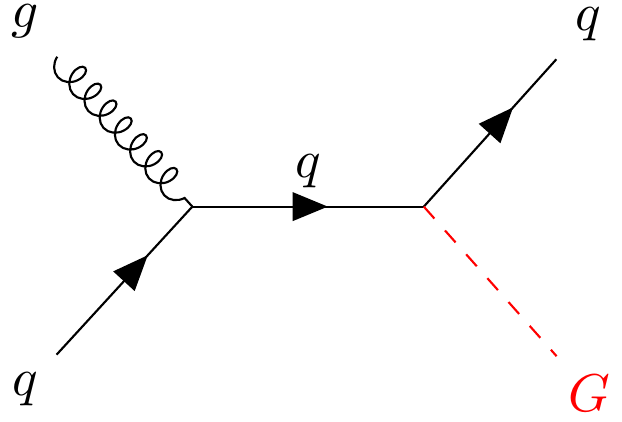
\includegraphics[width=\linewidth]{qg_to_qG}
    \caption{$q g \rightarrow q G$.}
  \end{subfigure}
  \begin{subfigure}{.48\linewidth}
    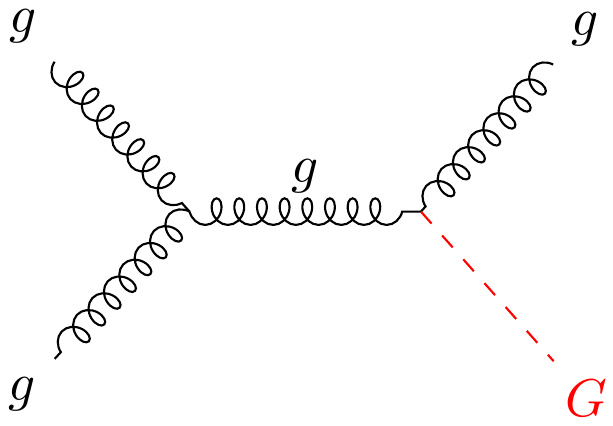
\includegraphics[width=\linewidth]{gg_to_gG}
    \caption{$g g \rightarrow g G$.}
  \end{subfigure}
  \caption{The main s-channel graviton production mechanisms for the \gls{add}
    model at \gls{lhc}.}
  \label{fig:add_feynman}
\end{figure}
%%% Local Variables:
%%% mode: latex
%%% TeX-master: "../search_for_DM_LED_with_ATLAS"
%%% End:
